
%%%%%%%%%%%%%%%%%%%%%%% file typeinst.tex %%%%%%%%%%%%%%%%%%%%%%%%%
%
% This is the LaTeX source for the instructions to authors using
% the LaTeX document class 'llncs.cls' for contributions to
% the Lecture Notes in Computer Sciences series.
% http://www.springer.com/lncs       Springer Heidelberg 2006/05/04
%
% It may be used as a template for your own input - copy it
% to a new file with a new name and use it as the basis
% for your article.
%
% NB: the document class 'llncs' has its own and detailed documentation, see
% ftp://ftp.springer.de/data/pubftp/pub/tex/latex/llncs/latex2e/llncsdoc.pdf
%
%%%%%%%%%%%%%%%%%%%%%%%%%%%%%%%%%%%%%%%%%%%%%%%%%%%%%%%%%%%%%%%%%%%


\documentclass[runningheads,a4paper]{llncs}

\usepackage{amssymb}
\setcounter{tocdepth}{3}
\usepackage{graphicx}

\usepackage{url}
\urldef{\mailsa}\path|{syshen,yingqin,|
\urldef{\mailsb}\path|jmzhang,|
\urldef{\mailsc}\path|skli}@nudt.edu.cn|
\newcommand{\keywords}[1]{\par\addvspace\baselineskip
\noindent\keywordname\enspace\ignorespaces#1}

\newtheorem{algorithm}{Algorithm}

\begin{document}

\mainmatter  % start of an individual contribution

% first the title is needed
%\title{Lecture Notes in Computer Science:\\Authors' Instructions
%for the Preparation\\of Camera-Ready
%Contributions\\to LNCS/LNAI/LNBI Proceedings}
\title{CompSyn: A Tool for Automatically Synthesizing Decoders}

% a short form should be given in case it is too long for the running head
%\titlerunning{Lecture Notes in Computer Science: Authors' Instructions}

% the name(s) of the author(s) follow(s) next
%
% NB: Chinese authors should write their first names(s) in front of
% their surnames. This ensures that the names appear correctly in
% the running heads and the author index.
%
\author{ShengYu Shen%
%\thanks{Project 61070132 supported by National Natural Science Foundation of China.}%
\and Ying Qin\and JianMin Zhang\and SiKun Li}
%
\authorrunning{ShengYu Shen\and Ying Qin\and JianMin Zhang\and SiKun Li}
% (feature abused for this document to repeat the title also on left hand pages)

% the affiliations are given next; don't give your e-mail address
% unless you accept that it will be published
\institute{School of Computer, National University of Defense Technology, China\\
\mailsa\mailsb\mailsc\\
\url{http://www.ssypub.org/}}

%
% NB: a more complex sample for affiliations and the mapping to the
% corresponding authors can be found in the file "llncs.dem"
% (search for the string "\mainmatter" where a contribution starts).
% "llncs.dem" accompanies the document class "llncs.cls".
%

\toctitle{Lecture Notes in Computer Science}
\tocauthor{Authors' Instructions}
\maketitle


\begin{abstract}
CompSyn is a tool that automatically synthesizes a decoder circuit from an encoder and a predefined assertion.
This tool has two usage modes: the synthesis mode and the inferring mode.

\vspace{0.1cm}

When the correct assertion is known,
\textbf{the synthesis mode} is used to determine the existence of the decoder and generate it.
On the other hand,
when the assertion is not known,
\textbf{the inferring mode} is used to infer this assertion and generate all possible decoders.
To help the user select the correct decoder,
this mode also infers each decoder's precondition formula,
which represents all cases that lead to this decoder's existence.

\vspace{0.1cm}

Experimental results show that
this tool can infer assertions and generate decoders for several complex encoders,
including PCI-E and Ethernet,
and the human effort in specifying assertion is significantly reduced.

\keywords{Complementary Synthesis, Inferring Assertion, Craig Interpolation, Functional Dependency}
\end{abstract}


\section{Introduction}\label{sec_intro}
One of the most difficult tasks in designing communication and multimedia chips
is to design and verify the complex complementary circuit pair $(E,E^{-1})$,
in which the encoder $E$ transforms information into a format suitable for transmission and storage,
while its complementary circuit(or decoder) $E^{-1}$ recovers this information.

To facilitate this job,
we have proposed the complementary synthesis algorithm \cite{ShengYuShen:iccad09,ShengYuShen:tcad,ShengYuShen:tcad11,ShengYuShen:iccad11}
and developed the CompSyn tool to automatically synthesize the decoder circuit of an encoder.
This tool has two usage modes, the synthesis mode and the inferring mode.

When the correct assertion is known,
\textbf{the synthesis mode} determines the existence of the decoder \cite{ShengYuShen:tcad11} by iteratively checking whether the encoder's input letter can be uniquely determined by its output sequence,
and characterizes the decoder's Boolean function \cite{ShengYuShen:tcad} with Craig interpolation \cite{Craig}.

On the other hand,
to manually specify an assertion,
the user must read extensive documentation and often perform laborious trial-and-error process.
That is why we develop the inferring mode to infer the assertion automatically.
\textbf{The inferring mode} includes three steps:
\textbf{1)} Inferring the assertion \cite{ShengYuShen:iccad11} by detecting and removing all cases without decoders.
\textbf{2)} Using functional dependency \cite{funcdep} to decompose $R$,
the Boolean relation uniquely determining the encoder's input letter,
into all possible decoders \cite{ShengYuShen:tcad12}.
\textbf{3)} Inferring each decoder's precondition formula \cite{ShengYuShen:tcad12} that represents all cases leading to this decoder's existence,
to help the user select the correct decoder.

For example,
our most complex benchmark--the XFI encoder,
has 120 configuration pins.
Finding out their meaning and correct combination was a very difficult and lengthy process,
which I had already experienced when using the synthesis mode in \cite{ShengYuShen:iccad09}.
On the contrary,
for the two decoders discovered by the inferring mode,
their corresponding precondition formulas refer to only three pins,
in which only two have different values.
Therefore,
to select the correct decoder,
I only need to find out the meaning of these \textbf{TWO} configuration pins instead of all 120 configuration pins.
More detail can be found in the experimental results section,
which indicates that the inferring mode can always significantly save the human effort in specifying assertion and selecting decoder.

All the experimental results and programs can be downloaded from \url{http://www.ssypub.org}.

\textbf{The remainder of this paper is organized as follows}.
Section \ref{sec_arch} introduces the CompSyn tool's software architecture.
Section \ref{sec_syn} presents the synthesis mode,
while Section \ref{sec_infer} introduces the inferring mode.
Section \ref{sec_exp} presents the experimental results,
and lastly,
Section \ref{sec_conclude} provides the conclusion.

\section{The software architecture}\label{sec_arch}
The CompSyn tool is implemented in the OCaml language.
Its architecture is shown in Figure \ref{fig_arch},
which comprises the following major components:

\begin{figure}[b]
\centering
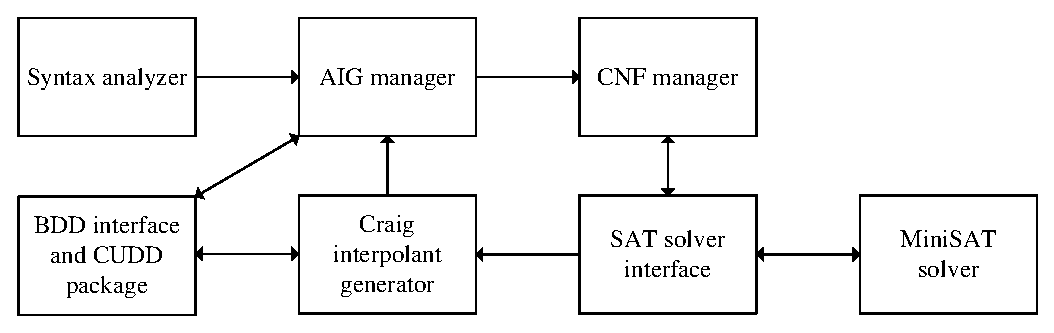
\includegraphics[width=0.8\textwidth]{arch}
\caption{The architecture of CompSyn}
\label{fig_arch}
\end{figure}

\subsection{Syntax analyzer}

This analyzer analyzes the encoder's Verilog source code and assertions,
and generates its transition relation's circuit description in an And-Inverter graph(AIG) \cite{aig}.

\subsection{AIG manager}

This AIG manager represents a circuit with an array.
% The access time of the array type in OCaml language is much faster than that of the list type,
% because it can be accessed directly with an integer index,
% while the access time of the list type is propositional to the list's length.
Elements of this array are of the following types:

\begin{enumerate}
\item TRUE: A logical constant true without parameter.
\item FALSE: A logical constant false without parameter.
\item VARIABLE: A node with an integer parameter,
which is this variable's encoding number.
\item INVERTER: An inverter with an integer parameter,
which refers to the index of the element that drives this inverter.
\item BUFFER:   A non-inverted buffer with an integer parameter,
which refers to the index of the element that drives this buffer.
\item AND: A two-input AND gate with two integer parameters that refer to the indexes of the elements that drive this AND gate.
\end{enumerate}

This AIG manager provides some procedures to manipulate the circuit represented in AIG,
such as removing redundant elements,
propagating constance,
and translating an AIG circuit to CNF formula.

\subsection{CNF manager}

This manager takes care of all CNF formulas generated by the syntax analyzer,
unrolled transition relations used to determine the existence of the decoder,
the formulas used to generate Craig interpolant,
and the formulas used to test functional dependency \cite{funcdep}.

The set of clauses of a CNF formula is stored in an OCaml list,
while each element of this list is another list that stores this clause's literal set.
The reasons for using list are that the clauses in a CNF formula do not need to be randomly accessed,
and the list type provides the flexibility to increase the size of the formula dynamically.

\subsection{The SAT solver interface and the SAT solver}

The SAT solver used here is the minisat solver v1.14 \cite{EXTSAT}.
This solver provides the ability to generate a proof for an unsatisfiable formula,
which can be analyzed to generate a Craig interpolant.

The proof generated by the minisat solver often includes most of the clauses appearing in the original formula,
which causes huge runtime overhead in generating Craig interpolant.
To reduce this overhead,
the minisat solver is modified to minimize the proof,
by removing those redundant clauses.

The OCaml to C interface that links CompSyn and minisat together is MiniSat-ocaml \cite{ocamlcbin} developed by Flavio Lerda.
However,
one of its major shortcomings is that it does not provide the ability to read back the proof from the minisat solver.
Hence,
such a procedure is added.

The other major shortcoming of this interface is that it only provides a procedure to allocate new variables one by one.
As the overhead of calling C procedure from OCaml is very high,
this will lead to very large runtime overhead for large formulas.
To reduce this overhead,
a new procedure that allocates all new variables in one calling is added.

\subsection{The Craig interpolant generator and the BDD interface}

The Craig interpolant generator works on the proof return from the minisat solver,
and generates the interpolant in AIG form.
One shortcoming of our Craig interpolant generator,
which is also shared by other implementations of the same algorithm \cite{interp_McMillan},
is that the generated interpolant contains lots of redundant gates.

To remove these redundant gates,
the CUDD package is invoked to generate a canonical representation of the interpolant.
The OCaml to C interface that links CUDD to CompSyn is taken from Blast model checker \cite{blast}.

After the simplification,
the BDD is converted back to a much more compact AIG by enumerating all cubes of this BDD.

\section{An overview of the synthesis mode}\label{sec_syn}

The overall flow of the synthesis mode is shown in Figure \ref{fig_halting}.
The loop iteratively increases the window size and unrolls the transition relation on that window.
Each iteration determines the decoder's existence by checking the $PC$ condition,
and determine the decoder's nonexistence by checking the $LN$ condition.
These two conditions will be introduced intuitively in the following subsections.

\begin{figure}[t]
\centering
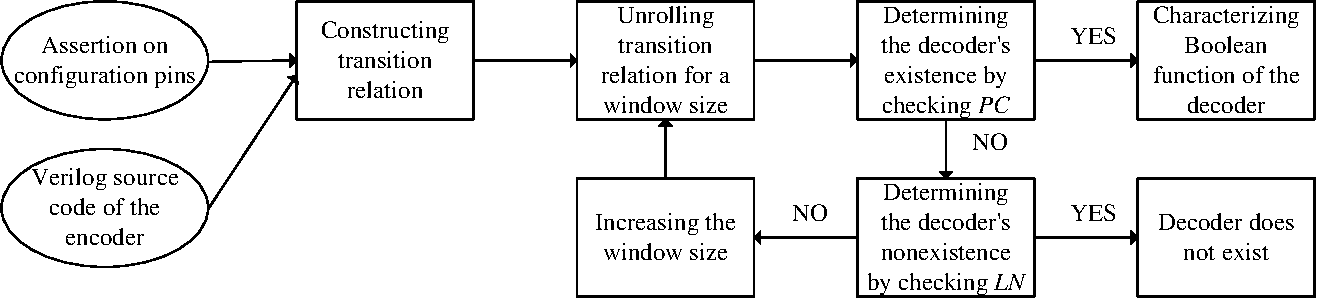
\includegraphics[width=\textwidth]{halting}
\caption{The flow of the synthesis mode}
\label{fig_halting}
\end{figure}

\subsection{Constructing transition relation}

This step takes two inputs,
one is the encoder's Verilog source code,
the other is the assertion on the encoder's configuration pins.
Normally,
an encoder has several modes,
each of which corresponds to a non-overlapped state set:

One of the most important modes is the working mode,
in which the encoder encodes its input.
Hence,
the encoder's input can be determined by its output,
which leads to the existence of its decoder.

On the other hand,
the encoder still has many other non-working modes,
such as the testing and sleep mode,
in which the encoder processes test commands or does nothing,
respectively.
Therefore,
in these modes,
the encoder's input cannot be determined by its output,
which leads to the nonexistence of its decoder.

Therefore,
the user needs to specify an assertion here to constrain the correct value of the encoder's configuration pins,
such that the encoder can be put in the correct working modes.


% \begin{figure}[t]
% \begin{center}
% 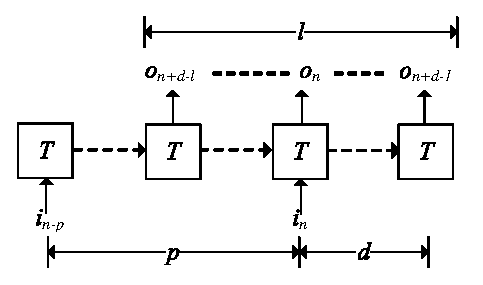
\includegraphics{t1}
% \end{center}
% \caption{The parameterized complementary condition}
%   \label{t1}
% \end{figure}
%
% \begin{figure}[b]
% \begin{center}
% 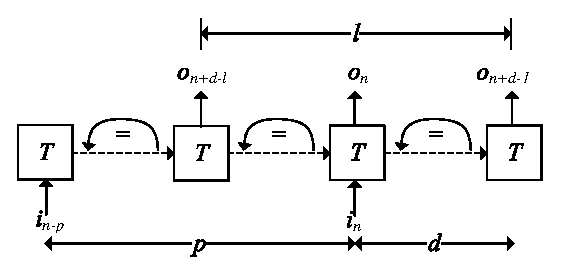
\includegraphics{doubleloop}
% \end{center}
% \caption{The loop-like non-complementary condition}
%   \label{doubleloop}
% \end{figure}

\subsection{Unrolling the transition relation and checking $PC$}

\begin{figure}[t]
\begin{center}
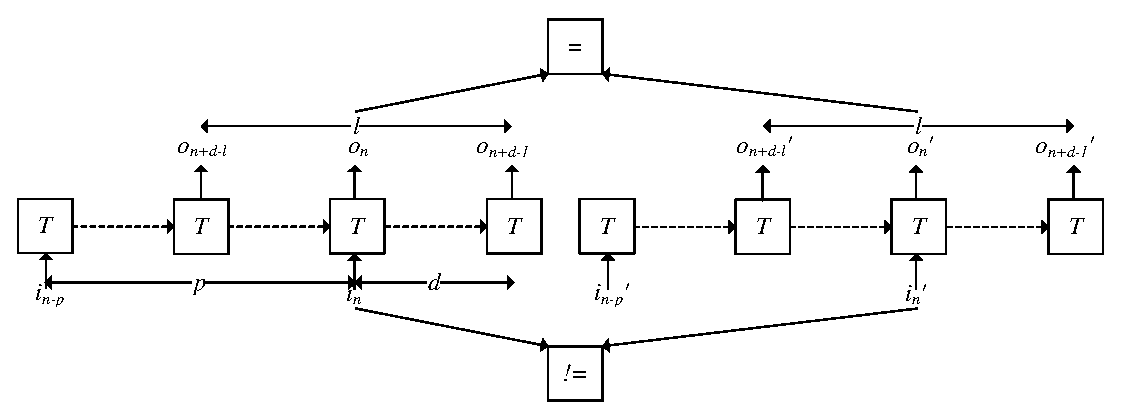
\includegraphics[width=\textwidth]{pc}
\end{center}
\caption{The $PC$ condition}
  \label{fig_pc}
\end{figure}

$PC$ is the abbreviation of Parameterized Complementary Condition defined in \cite{ShengYuShen:iccad09},
which is used to determine the existence of the decoder.
Its meaning is intuitively shown in Figure \ref{fig_pc},
where $T$ is the encoder's transition relation constructed in the previous step,
while $i_n$ and $o_n$ are the input and output letter,
respectively,
and $p$, $d$, and $l$ are the lengths of the unfolded transition relation,
which are also called \textbf{the window size}.

This figure,
and therefore $PC$,
indicates that the decoder exists if and only if there exists $p$, $d$, and $l$,
such that the output sequence $<o_{n+d-l},\dots,o_{n+d-1}>$ can uniquely determine the input letter $i_n$.
In other words,
there does not exist two different input letters $i_n$ and $i_n'$ that can be recovered from the same output sequence $<o_{n+d-l},\dots,o_{n+d-1}>$.

This condition can be encoded into a SAT instance and solved with the minisat solver \cite{EXTSAT}.
If the result is unsatisfiable,
then the decoder exists;
otherwise,
the decoder does not exist for this particular value of $p$, $d$, and $l$.
CompSyn needs to check $LN$ or increase the window size.

\subsection{Checking $LN$}
\begin{figure}[t]
\begin{center}
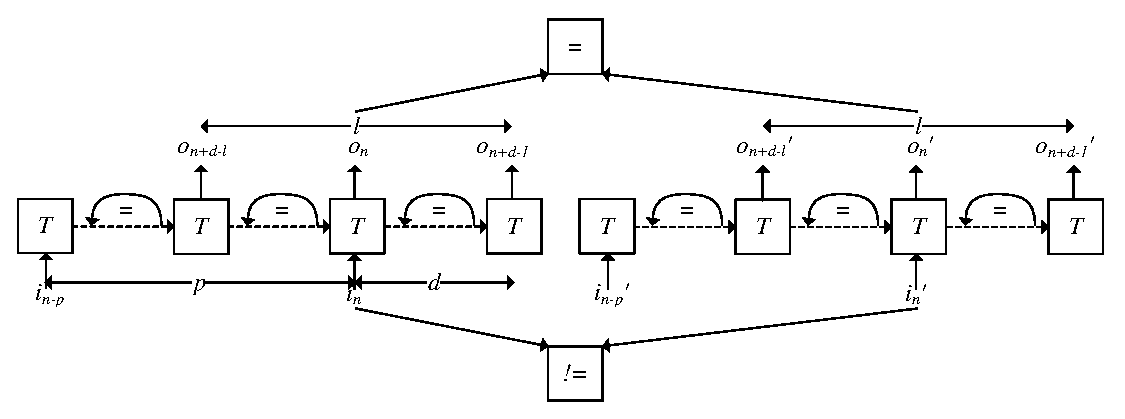
\includegraphics[width=\textwidth]{ln}
\end{center}
\caption{The $LN$ condition}
  \label{fig_ln}
\end{figure}

In addition to the $PC$ mentioned in the last subsection,
another condition $LN$ had been defined in \cite{ShengYuShen:tcad11} to determine the nonexistence of the decoder.
Its meaning is intuitively shown in Figure \ref{fig_ln},
indicating that the decoder does not exist if and only if there exists $p$, $d$, and $l$,
such that the output sequence $<o_{n+d-l},\dots,o_{n+d-1}>$ can \textbf{NOT} uniquely determine the input letter $i_n$,
and there are three loops on state sequences $<s_{n-p},\dots,s_{n+d-l}>$,$<s_{n+d-l+1},\dots,s_n>$, and $<s_{n+1},\dots,s_{n+d}>$.

This condition can be encoded into a SAT instance,
and solved with the minisat solver \cite{EXTSAT}.
If this SAT instance is satisfiable,
then the nonexistence of the decoder for all those longer paths can be proved by unfolding these loops.
Otherwise,
the window size will be increased and a new iteration will begin.
We have proven in \cite{ShengYuShen:tcad11} that the loop between $LN$ and $PC$ will eventually terminate.



\subsection{Characterizing the Boolean function of the decoder}

If the $PC$ checking succeeds,
then there exists a function that maps the output sequence $<o_{n+d-l},\dots,o_{n+d-1}>$ back to the input letter $i_n$.
This function can be characterized from the Boolean relation shown in Figure \ref{fig_pc},
with the ALLSAT algorithm proposed in \cite{ShengYuShen:tcad}.

Recently,
Liu et al. \cite{Roland:iccad11} proposed a much faster algorithm based on Craig interpolant \cite{Craig} to characterize this function.
The timing and area of the decoder generated by it is comparable to our ALLSAT algorithm.

This algorithm had also been implemented in CompSyn.
%whose major idea is shown intuitively in Figure \ref{fig_craig}.
To simplify the presentation,
we denote $i_n$ as $Y$,
the $j$-th bit of $Y$ as $Y^{j}$,
and $<o_{n+d-l},\dots,o_{n+d-1}>$ as $X$.
$R(X,Y)$ is the Boolean relation shown in Figure \ref{fig_pc},
which succeeds in checking $PC$.
As $R$ can uniquely determine the value of $Y$ from $X$,
a Craig interpolant of $R(X,Y)\wedge Y^{j}\equiv 1$ with respect to $R(X,Y')\wedge Y'^{j} \equiv 0$ can be generated.
This Craig interpolant is exactly the Boolean function that computes the $j$-th bit of $Y$ from $X$.
%\begin{figure}[b]
%\begin{center}
%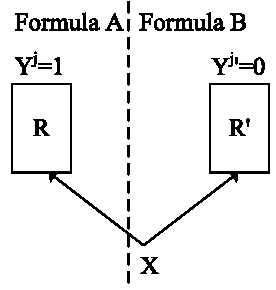
\includegraphics[width=0.15\textwidth]{craig}
%\end{center}
%\caption{Characterizing the Boolean function of the decoder with Craig interpolant}
%  \label{fig_craig}
%\end{figure}



\section{An overview of the inferring mode}\label{sec_infer}
To manually specify an assertion,
the user must read extensive documentation
and often perform laborious trial-and-error process.
This is why we develop the inferring mode that infers the assertion automatically.

The flow of the inferring mode is shown in Figure \ref{fig_infer}.
It is similar to Figure \ref{fig_halting},
with some new steps in gray color.
The assertion can be automatically inferred in this mode,
so the user does not need to specify it here.

One major difference while compared to the synthesis mode is the inner loop on the Checking $LN$ step.
Because the Checking $LN$ step can find out a configuration pin value that leads to the decoder's nonexistence,
a new step is inserted after it to remove all such values,
to ensure all remained configuration pin values have corresponding decoders.

The other major difference is the addition of two steps after the outer loop.
Because the inferred assertion actually includes multiple configuration pin values,
there may simultaneously exist multiple decoders.
Therefore,
a new step is inserted to discover all of them,
and another step is inserted to infer a precondition formula for each decoder,
which represents the set of configuration values that can lead to this decoder's existence.

\begin{figure}[t]
\centering
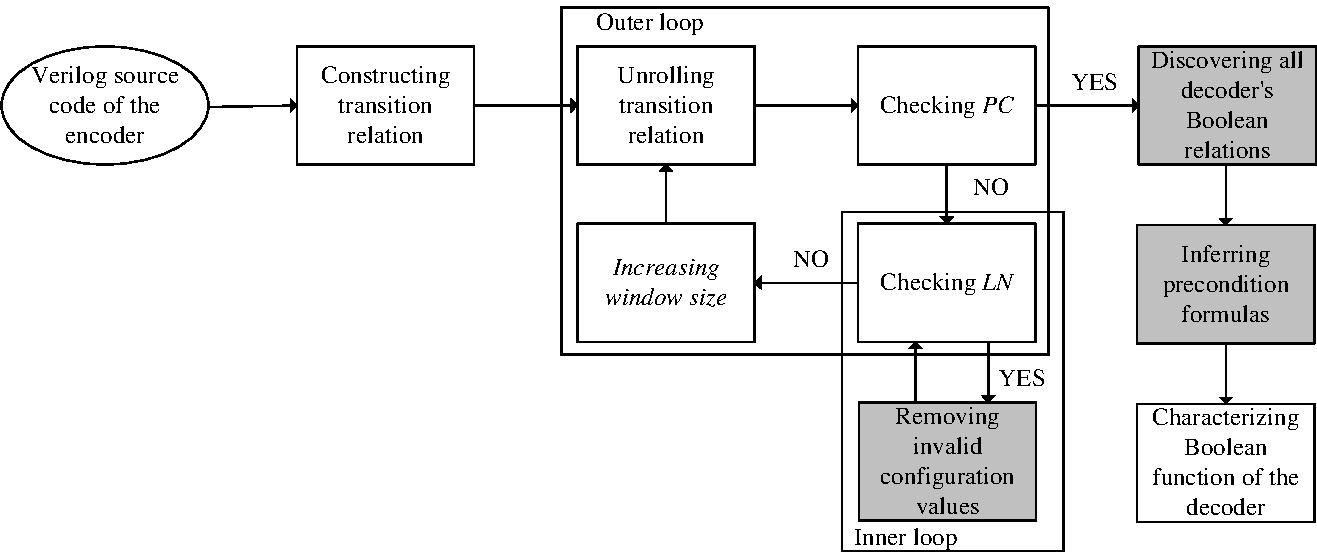
\includegraphics[width=\textwidth]{infer}
\caption{The flow of the inferring mode}
\label{fig_infer}
\end{figure}


\subsection{Ruling out invalid configuration values}

If the $LN$ checking succeeds,
an invalid configuration value that leads to the nonexistence of the decoder can be obtained from the  minisat \cite{EXTSAT} solver's satisfying assignment.
We can simply rule out this invalid configuration value and return to the previous step to check $LN$ again.
However,
to reduce the runtime overhead,
an algorithm has been proposed in \cite{ShengYuShen:iccad11} to enlarge this value to a larger set of invalid configuration values with Craig interpolant \cite{Craig},
such that they can be rule out altogether.
\begin{figure}[t]
\centering
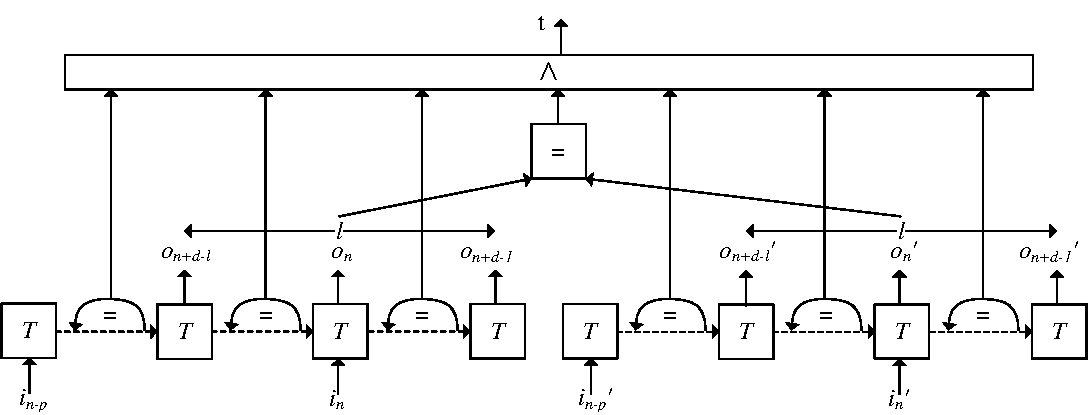
\includegraphics[width=\textwidth]{lninfer}
\caption{Enlarging the invalid configuration value with Craig interpolant}
\label{fig_lninfer}
\end{figure}

The formula used in enlarging is shown in Figure \ref{fig_lninfer}.
It is very similar to that of Figure \ref{fig_ln},
except that the existence of the six loops and the equality of the two output sequences are conjuncted together to generate a new Boolean variable $t$.
By assigning all $i_n$'s and $i_n'$'s satisfying assignment to Figure \ref{fig_lninfer},
this formula can be transformed into a new formula $F(c,t)$,
which defines a circuit,
whose input is the configuration value $c$,
and output is $t$.

The Boolean function of this circuit can be characterized by generating the Craig interpolant of $F(c,1)$ with respect to $F(c,0)$.
Thus,
this Boolean function is exactly the enlarged set of invalid configuration values.


The inner loop between this step and the Checking $LN$ step will eventually terminate after such invalid configuration values are all ruled out.
Then,
the window size is increased to check $PC$ again.



We have proven in \cite{ShengYuShen:iccad11} that the outer loop between $LN$ and $PC$ will eventually terminate.
Assume that the set of all configuration values ruled out is $NA$,
then the final inferred assertion is $\wedge_{na\in NA}\neg na$.

\subsection{Discovering all decoders' Boolean relations}

\begin{figure}[b]
\centering
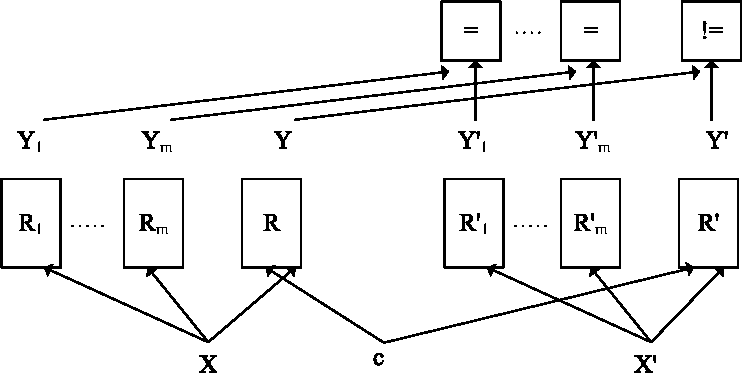
\includegraphics[width=0.7\textwidth]{fdtest_dec}
\caption{The SAT instance that discovers all decoders}
\label{fig_fdtest_dec}
\end{figure}

The final inferred assertion is a formula that actually contains many different configuration values.
This means that multiple decoders may exist simultaneously for this inferred assertion.
Thus,
we need to find out the set of all decoders' step by step.

We denote $i_n$ as $Y$,
$<o_{n+d-l},\dots,o_{n+d-1}>$ as $X$,
and the configuration value as $c$.
Then $R(c,X,Y)$ is the Boolean relation shown in Figure \ref{fig_pc} that succeeds in checking $PC$.

Assume $\{R_1,\dots,R_{m}\}$ is a set of decoders' Boolean relations that has already been discovered.
To test whether all decoders have already been discovered,
the SAT instance shown in Figure \ref{fig_fdtest_dec} is constructed based on functional dependency \cite{funcdep}.

% In Figure \ref{fig_fdtest_dec},


According to \cite{ShengYuShen:tcad12},
if this SAT instance is unsatisfiable,
then $Y$ can be uniquely determined by $\{Y_1,\dots,Y_m\}$,
which means all decoders have been discovered.
Otherwise,
a new decoder's Boolean relation can be discovered by assigning the satisfying assignment of $c$ to $R$.

A new round of functional dependency test will be performed again,
until no more decoder can be discovered.
Subsequently,
these Boolean relations will be used to characterize their corresponding decoders' Boolean functions,
with the ALLSAT algorithm \cite{ShengYuShen:tcad} or the one based on Craig interpolation \cite{Roland:iccad11}.

\subsection{Inferring precondition formulas}
\begin{figure}[b]
\centering
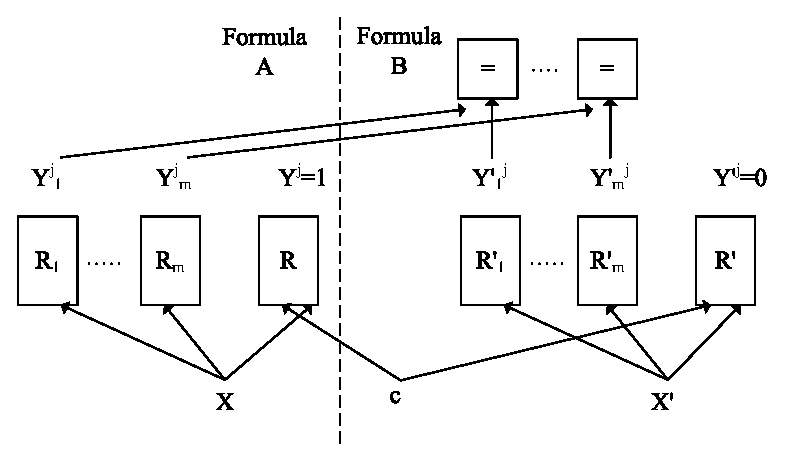
\includegraphics[width=0.7\textwidth]{fdtest_infer}
\caption{The SAT instance that infers precondition formulas}
\label{fig_fdtest_infer}
\end{figure}

Assume that $\{R_1,\dots,R_{m}\}$ is the set of all decoders' Boolean relations discovered in the last step,
and $\{IA_1,\dots,IA_{m}\}$ is their corresponding set of configuration letters.
To help the user determine which $R_i$ in $\{R_1,\dots,R_{m}\}$ is the correct decoder,
each $IA_i$ in $\{IA_1,\dots,IA_{m}\}$ must be characterized.

Assume $Y$ and all $Y_i$ in Figure \ref{fig_fdtest_dec} are vectors of the same length $v$,
and their $j$-th bit are $Y^{j}$ and $Y_i^{j}$,respectively.
If the precondition formulas $IA^j_i$ for the $j$-th bit of $IA_i$ can be characterized,
then $IA_i$ can be defined as $\bigwedge _{j=0}^{v-1} IA^j_i$.

To achieve this goal,
the unsatisfiable SAT instance shown in Figure \ref{fig_fdtest_infer} is constructed.
This SAT instance is very similar to that of Figure \ref{fig_fdtest_dec},
except that only the $j$-th bit is constrained.
Therefore it is unsatisfiable.
% which represents a functional dependency problem \cite{funcdep}.
As the set of common variables between formula $A$ and $B$ is $\{c, Y_1^j, \dots, Y_m^j\}$,
the generated interpolant of $A$ with respect to $B$ is a function $F(c,Y_1^j, \dots, Y_m^j)$ that computes the value of $Y^j$.
By setting the value of $Y_i^j$ to 1 and all other $\{Y_k^j|k\ne i\}$ to 0 in $F(c,Y_1^j, \dots, Y_m^j)$,
we can obtain the formula $IA^j_i$.
%\begin{figure}[t]
%\centering
%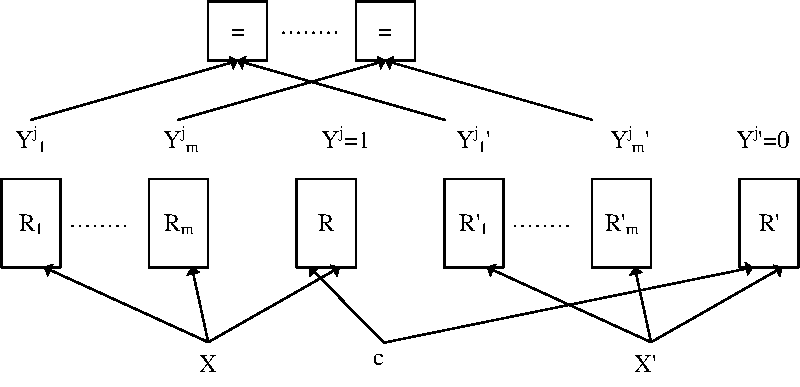
\includegraphics[width=0.75\textwidth]{fdtest_simple}
%\caption{The SAT instance that infers precondition formulas}
%\label{fig_fdtest_simple}
%\end{figure}



\section{Experimental results}\label{sec_exp}
\subsection{The usage model}
All these steps mentioned above are connected together by the standard make tool in Linux.
To use the synthesis mode,
the user needs to run the command "make halting" under the bash shell in the benchmark directory.
To use the inferring mode,
the user needs to run the command "make infer\_multidec\_not\_charfirst \_nowall".

\subsection{Benchmarks}
The benchmarks used in the experiments include several complex encoders from industrial projects,
\begin{enumerate}
\item A XGXS encoder compliant to clause 48 of IEEE-802.3ae 2002 standard \cite{IEEE80232002}.
\item A XFI encoder compliant to clause 49 of the same IEEE standard.
\item A 66-bit scrambler used to ensure
that a data sequence has sufficient 0-1 transitions,
so that it can run through a high-speed
noisy serial transmission channel.
\item A PCI-E physical coding module \cite{PCIESPEC}.
\item The Ethernet module of Sun's OpenSparc T2 processor.
\end{enumerate}

The profiles of these benchmarks are shown in Table \ref{tab_benchmark}.
Some of these large benchmarks have more than 1000 lines of source code,
while the XFI encoder has more than 100 state variables and configuration pins.


\begin{table}[t]
\centering
\caption{Information on Benchmarks}
\begin{tabular}{|c|c|c|c|c|c|}
\hline
&XGXS&XFI&scrambler&PCIE&T2 Ethernet\\\hline\hline
Line number&&&&&\\
of verilog&214&466&24&1139&1073\\
source code&&&&&\\\hline
\#state variables&15&135&58&22&48\\\hline
Data path width&8&64&66&10&10\\\hline
\end{tabular}\label{tab_benchmark}
\end{table}

\subsection{The experimental result of the synthesis mode}
\begin{table}[t]
\centering
\caption{Experimental results on the correct and incorrect encoders}
\begin{tabular}{|c|c|c|c|c|c|c|}
\hline
&                                        &XGXS     &XFI       &scrambler     &PCI-E    &T2 Ethernet\\ \hline\hline
% &Time to ch-                           &&&&&\\
% \cite{ShengYuShen:fmcad10}&eck $PC$(sec) &1.06     &70.52     &5.74      &2.40    &66.37\\\cline{2-7}
% &$d,p,l$                                 &1,1,1    &0,3,2     &0,2,2     &2,1,1   &4,1,1         \\ \hline\hline
For &Time to check the                         &&&&&\\
correct&decoder's existence(sec)                      &0.29     &17.86     &2.67      &0.47    &29.64\\\cline{2-7}
%      &improve \%                         &72.64    &74.67     &53.48     &80.42   &55.34 \\\cline{2-7}
encoder&$d,p,l$                                 &1,2,1    &0,3,2     &0,2,2     &2,2,1   &4,4,1          \\ \hline\hline
For&Time to check the                          &&&&&\\
incorrect&decoder's existence(sec)             &0.16     &7.59     &1.17      &0.33    &2.19\\
encoder&                        &&&&&\\\hline

\end{tabular}\label{tab_prodes}
\end{table}

According to Table \ref{tab_prodes} and \cite{ShengYuShen:tcad11},
when given the assertion,
%no matter correct or not,
the synthesis mode can determine the existence of the decoders within 40 seconds,
and builds the decoders within 10 seconds with an algorithm similar to that of Liu et al. \cite{Roland:iccad11}.

Moreover,
we inserted some bugs into these encoders,
which generated the same output letter for two different input letters.
CompSyn successfully detected all these bugs within 10 seconds.

\subsection{The experimental result of the inferring mode}
\begin{table}[b]
\centering
\caption{Experimental Results of the inferring mode}
\begin{tabular}{|c|c|c|c|c|c|c|}
\hline
                                        &XGXS     &XFI       &scrambler     &PCI-E    &T2 Ethernet\\\hline\hline
Config                 &&&&&\\
pin number                              &3        &120       &1             &16      &26\\\hline
Runtime                                 &3.83     &3841.34   &18.73         &8.51    &1791.22      \\\hline
$d,p,l$                                 &1,5,1    &0,5,2     &0,4,2         &2,5,1   &4,5,1          \\ \hline
Number of                               &&&&&          \\
decoders                                &1        &2         &2             &1       &1          \\ \hline
\end{tabular}\label{tab_res}
\end{table}

According to Table 	\ref{tab_res},
when the assertions are not known,
the inferring mode can infer assertions, generate decoders and infer these decoders' precondition formulas within 4000 seconds.

The set of inferred assertions are shown below:

\textbf{For XGXS}:
\texttt{( ( !bad\_code ) )}

\textbf{For XFI}:
\texttt{( ( TEST\_MODE ) | ( !TEST\_MODE \& RESET ) | ( !TEST\_MODE \& !RESET \& DATA\_VALID ) )}

\textbf{For scrambler}:
\texttt{True}

\textbf{For PCI-E}:
\texttt{( ( !TXELECIDLE \& CNTL\_TXEnable\_P0 \& CNTL\_RESETN\_P0 \& !CNTL\_Loopback\_P0 ) )}

\textbf{For T2 ethernet}:
\texttt{( ( link\_up\_loc \& !reset\_tx \& !txd\_sel[1] \& !jitt er\_study\_pci[1] \& !txd\_sel[0] \& !jitter\_study\_pci[0] ) | ( !link\_up\_l oc \& !reset\_tx \& !txd\_sel[1] \& tx\_enc\_conf\_sel[3] \& tx\_enc\_conf\_sel[2] \& !jitter\_study\_pci[1] \& !txd\_sel[0] \& !jitter\_study\_pci[0] ) | ( !l ink\_up\_loc \& !reset\_tx \& !txd\_sel[1] \& tx\_enc\_conf\_sel[3] \& !tx\_enc\_conf \_sel[2] \& tx\_enc\_conf\_sel[1] \& !jitter\_study\_pci[1] \& !txd\_sel[0] \& !ji tter\_study\_pci[0] ) | ( !link\_up\_loc \& !reset\_tx \& !txd\_sel[1] \& !tx\_ enc\_conf\_sel[3] \& !tx\_enc\_conf\_sel[2] \& tx\_enc\_conf\_sel[1] \& !jitter\_ study\_pci[1] \& !txd\_sel[0] \& !jitter\_study\_pci[0] \& tx\_enc\_conf\_sel[0] ) )}

Moreover,
only two out of the five benchmarks have two decoders,
while the other three have only one decoder.
This means that,
in most cases,
our algorithm generates only one decoder.
For other cases with multiple decoders,
the user needs to inspect the inferred precondition formulas to select the correct one.

For the two decoders of scrambler,
their corresponding precondition formulas are $reset$ and $!reset$.
By inspecting the Verilog source code of scrambler,
we found that the $reset$ is used to reset the scrambler when it is $True$.
Thus,
the scrambler encoder will work in normal mode when $reset$ is $False$.
Therefore,
the second decoder is the correct one.
And the dynamic simulation had confirmed its correctness.


For the two decoders of the most complex XFI encoder \cite{IEEE80232002},
their corresponding precondition formulas are $RESET~\& !TEST\_MODE~\&~!DATA\_VALID$ and $!RESET~\&~!TEST\_MODE~\&~DATA\_VALID$.
The only differences between them are the value of $RESET$ and $DATA\_VALID$.
By inspecting the Verilog source code of XFI,
we found that the $RESET$ is used to reset the XFI encoder when it is $True$,
and $DATA\_VALID$ means that the input data is valid when it is $True$.
So,
the XFI encoder will work in normal mode when $RESET$ is $False$ and $DATA\_VALID$ is $True$.
Therefore,
the second decoder is the correct one.
The dynamic simulation had also confirmed its correctness.

In this process,
the user only needs to inspect the meaning of two configuration pins,
instead of all 120 configuration pins of the XFI encoder.
In this way,
the human effort in specifying assertion and selecting the correct decoder is significantly reduced.

\section{Conclusions}\label{sec_conclude}
The CompSyn tool can infer correct assertions and generate decoder circuits for several complex encoders.
Furthermore,
it can significantly reduce the human effort in specifying assertion and selecting the correct decoder.


% \section*{Acknowledgment}
% The authors would like to thank the anonymous reviewers for their hard work.

% This work was funded by Projects 60603088 and 61070132 supported by National Natural Science Foundation of China.

\begin{thebibliography}{4}

\bibitem{ShengYuShen:iccad09}
ShengYu Shen, Jianmin Zhang, Ying Qin, Sikun Li: Synthesizing complementary circuits automatically. ICCAD 2009: 381-388


\bibitem{ShengYuShen:tcad}
ShengYu Shen, Ying Qin, KeFei Wang, LiQuan Xiao, Jianmin Zhang, Sikun Li: Synthesizing Complementary Circuits Automatically. IEEE Trans. on CAD of Integrated Circuits and Systems 29(8): 1191-1202 (2010)


\bibitem{ShengYuShen:tcad11}
ShengYu Shen, Ying Qin, LiQuan Xiao, KeFei Wang, Jianmin Zhang, Sikun Li: A Halting Algorithm to Determine the Existence of the Decoder. IEEE Trans. on CAD of Integrated Circuits and Systems 30(10): 1556-1563 (2011)


\bibitem{ShengYuShen:iccad11}
ShengYu Shen, Ying Qin, Jianmin Zhang, Sikun Li: Synthesizing complementary circuits automatically.
\emph{accepted by ICCAD11}.

\bibitem{ShengYuShen:tcad12}
ShengYu Shen, Ying Qin, LiQuan Xiao, KeFei Wang, Jianmin Zhang, Sikun Li: Inferring Assertion for Complementary Synthesis.
submitted to IEEE transaction on CAD of Integrated Circuits and Systems.

\bibitem{Roland:iccad11}
Siou-Yuan Liu,
Yen-Cheng Chou,
Chen-Hsuan Lin,
Jie-Hong Roland Jiang
:
Completely Automatic Decoder Synthesis.
\emph{accepted by ICCAD11}.


% \bibitem{Cofact}
% Ganai, M.K.,
% Gupta, A.,
% Ashar, P.
% :
% Efficient SAT-based unbounded symbolic model checking using circuit cofactoring.
% In: 2004 International Conference on Computer-Aided Design,
% pp. 510--517.
% IEEE Press,
% New York (2004)


\bibitem{Craig}
William Craig,
:
Linear reasoning: A new form of the Herbrand-Gentzen theorem.
J. Symbolic Logic. 22(3), 250--268 (1957)


\bibitem{EXTSAT}
Niklas E\'en, Niklas S\"orensson: An Extensible SAT-solver. SAT 2003: 502-518


\bibitem{PCIESPEC}
PCI Express Base Specification Revision 1.0.
\url{http://www.pcisig.com}

\bibitem{IEEE80232002}
\emph{IEEE Standard for Information technology Telecommunications and
  information exchange between systems Local and metropolitan area networks
  Specific requirements Part 3: Carrier Sense Multiple Access with Collision
  Detection (CSMA/CD) Access Method and Physical Layer Specifications
  Amendment: Media Access Control (MAC) Parameters, Physical Layers, and
  Management Parameters for 10 Gb/s Operation}, IEEE Std. 802.3, 2002.

\bibitem{funcdep}
Chih-Chun Lee, Jie-Hong Roland Jiang, Chung-Yang Huang, Alan Mishchenko: Scalable exploration of functional dependency by interpolation and incremental SAT solving. ICCAD 2007: 227-233

\bibitem{aig}
Alan Mishchenko, Satrajit Chatterjee, Robert K. Brayton: DAG-aware AIG rewriting a fresh look at combinational logic synthesis. DAC 2006: 532-535

\bibitem{ocamlcbin}
\url{https://github.com/flerda/MiniSat-ocaml/wiki}


% \bibitem{CHAFF}
% Moskewicz, M.,
% Madigan, C.,
% Zhao, Y.,
% Zhang, L.,
% Malik, S.
% :
% Chaff: Engineering an Efficient SAT Solver.
% In: 38th Design Automation Conference,
% pp. 530--535.
% IEEE Press,
% New York (2001)



% \bibitem{grasp}
% Silva, J.,
% Sakallah, K.
% :
% GRASP - a new search algorithm for satisfiability.
% In: 1996 International Conference on Computer-Aided Design,
% pp. 220--227.
% IEEE Press,
% New York (1996)


% \bibitem{BERKMIN}
% Goldberg, E.,
% Novikov, Y.
% :
% BerkMin: A Fast and Robust Sat-Solver.
% In: 2002 Design, Automation and Test in Europe Conference and Exposition,
% pp. 142--149.
% IEEE Press,
% New York (2002)


% \bibitem{interp_Krajicek} Krajicek, J.: Interpolation theorems, lower bounds for proof systems,
% and independence results for bounded arithmetic.
% J. Symbolic Logic 62(2), 457--486 (1997)


% \bibitem{interp_Pudlak} Pudlak, P.: Lower bounds for resolution and cutting plane proofs and
% monotone computations.
% J. Symbolic Logic 62(3), 981--998 (1997)


\bibitem{interp_McMillan}
Kenneth L. McMillan: Interpolation and SAT-Based Model Checking. CAV 2003: 1-13

\bibitem{blast}
Dirk Beyer, Thomas A. Henzinger, Ranjit Jhala, Rupak Majumdar: The software model checker Blast. STTT 9(5-6): 505-525 (2007)


% \bibitem{MEALY} Mealy, G.H.: A method for synthesizing sequential circuits.
% Bell Systems Technical Journal 34(5), 1045--1079 (1955)

% \bibitem{RecDiam}
% Kroening, D.,
% Strichman, O.
% :
% Efficient Computation of Recurrence Diameters.
% In: Zuck, L.D., Attie, P.C., Cortesi, A., Mukhopadhyay, S. (eds.)
% VMCAI 2003.
% LNCS, vol. 2575,
% pp. 298--309.
% Springer, Heidelberg (2003)

% \bibitem{ShengYuShen:fmcad10}
% Shen, S.,
% Qin, Y.,
% Zhang, J.,
% Li, S.
% :
% A Halting Algorithm to Determine the Existence of Decoder.
% In: 10th International Conference on Formal Methods in Computer-Aided Design,
% pp. 91--100.
% IEEE Press,
% New York (2010)

% \bibitem{dim_syn}
% Gulwani, S.
% :
% Dimensions in program synthesis.
% In: 12th International ACM SIGPLAN Conference on Principles and Practice of Declarative Programming,
% pp. 13--24.
% ACM Press,
% New York (2010)
%
% \bibitem{prog_inv}
% Edsger W. Dijkstra.
% Program Inversion.
% in Program Construction,
% pp 54-57,
% 1978.
%
%
% \bibitem{mtd_autoProginv}
% Gl\"{u}ck, R.,
% Kawabe, M.
% :
% A method for automatic program inversion based on LR(0) parsing.
% Fundam. Inf. 66(4), 367--395 (2005)
%
% \bibitem{prog_inv_rev}
% Srivastava, S.,
% Gulwani, S.,
% Chaudhuri, S.,
% Foster, J.
% :
% Program inversion revisited.
% Technical Report MSR-TR-2010-34, Microsoft Research (2010)
%
%
%
% \bibitem{converter_date08}
% Avnit, K.,
% D'Silva, V.,
% Sowmya, A.,
% Ramesh, S.,
% Parameswaran, S.
% :
% A Formal Approach To The Protocol Converter Problem.
% In: 2008 Design, Automation and Test in Europe Conference and Exposition,
% pp. 294--299.
% IEEE Press,
% New York (2008)
%
%
% \bibitem{converter_date09}
% Avnit, K.,
% Sowmya, A.
% :
% A formal approach to design space exploration of protocol converters.
% In: 2009 Design, Automation and Test in Europe Conference and Exposition,
% pp. 129--134.
% IEEE Press,
% New York (2009)


% \bibitem{converter_tacas10}
% Avnit, K.,
% Sowmya, A.,
% Peddersen, J.
% :
% ACS: Automatic Converter Synthesis for SoC Bus Protocols.
% In: Esparza, J., Majumdar,R. (eds.)
% TACAS 2010.
% LNCS, vol. 6015,
% pp. 343--348.
% Springer, Heidelberg (2010)

\end{thebibliography}



\end{document}
